\section{Notification functions - Jacek}

Notification part is a very important part of our project. After collecting the data, preparing them and using machine learning algorithms, we need to somehow communicate with the user. In this paragraph we will describe the motivation and ways of informing the user about the anomalies and predictions.

\subsection{Motivation}
To notify the user in order to react for the main events such as anomaly detection, we created a notification functions. Firstly we are calling user by triggering ChatBot API and secondly we are sending notification to the slack channel with a graph and marked anomaly to let user faster react for it.

\textbf{User story} \\
We decided to create a user story where user who will be notified in case of an alert is one of the administrators Bob. Bob and his team are using slack in their work as we do in this project. \\
In case of the anomaly detection we are triggering ChatBot API to call Bob and notify him about the anomaly. To let Bob faster make his decision and in case of emergency, escalate the problem(or in case of false detection skip it), we decided to show to him the graph where he can visually asses the problem. Since Bob and his team are using slack we decided to send them notification to special slack channel as well. \\
To accelerate the decision making process, even before logging in to the consoles, cloud watches etc. we decided to send him a part of the graph with prediction and marked anomaly. This will be straightforward information for the Bob or his colleagues what is happening. The example of notification massages send to the slack channel is depicted in a fig. \ref{fig:userNotif}.

\begin{figure}[h!]
    \centering
    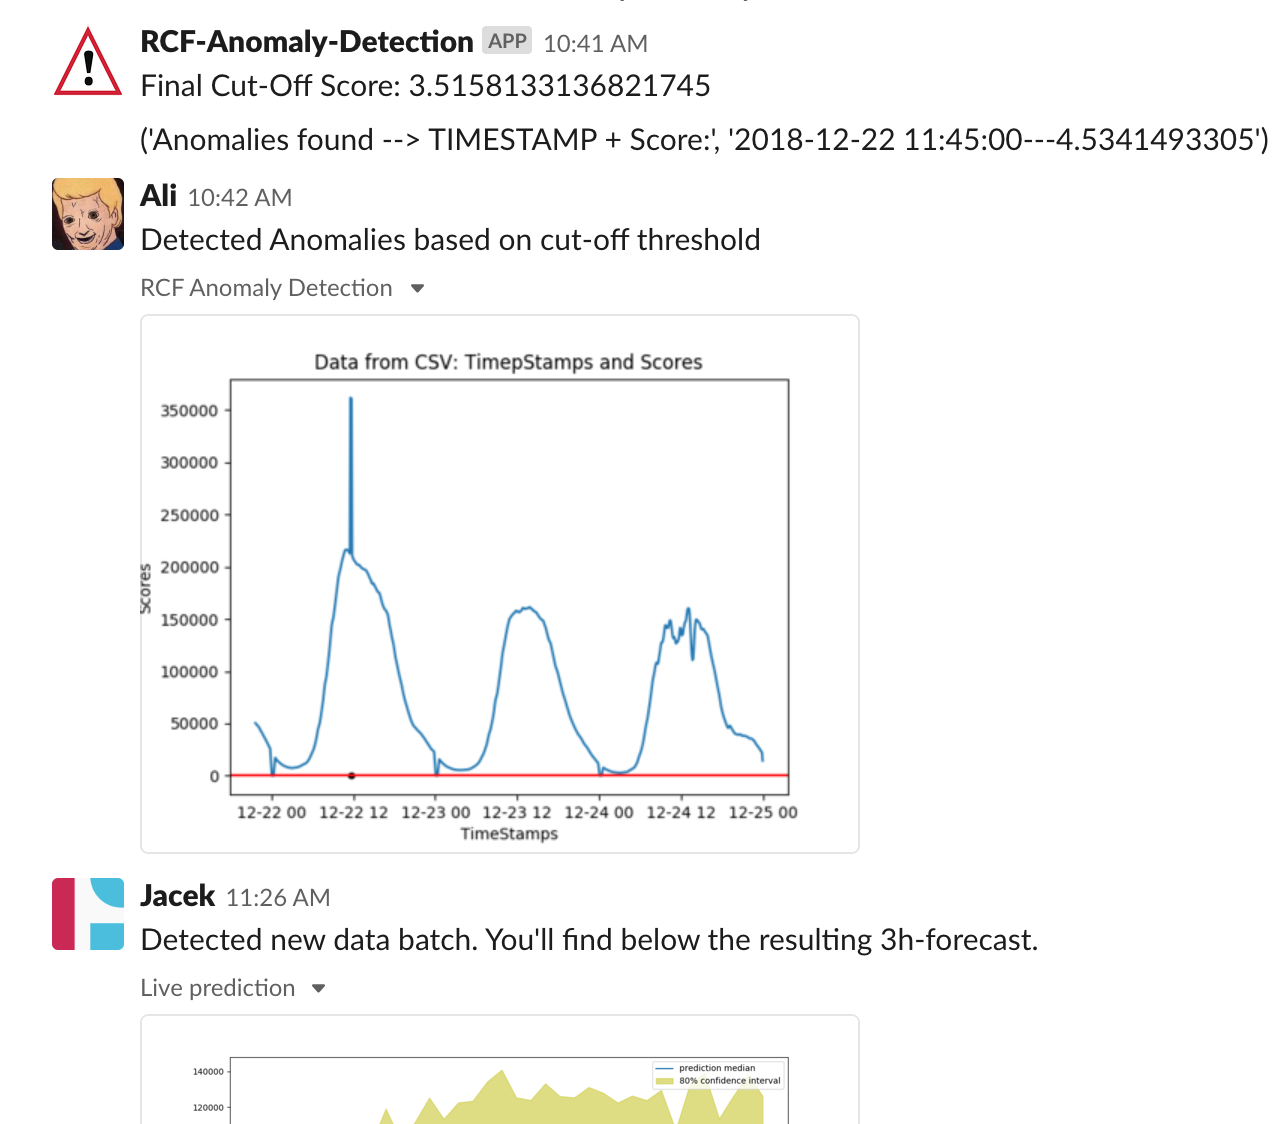
\includegraphics[width=0.8\textwidth]{images/UserNotification.png}
    \caption{Example of anomaly notification}
    \label{fig:userNotif}
\end{figure}

\subsection{Methods to notify the user about detected anomalies}
\begin{itemize}
\item \textbf{ChatBot API notification} - To notify the ChatBot API in case of an anomaly we are sending REST POST message to provided by ChatBot team URL as it is shown in an example in fig. \ref{fig:chatbot}. That POST is triggering ChatBot which calls the user.
\end{itemize}

\begin{figure}[h!]
    \centering
    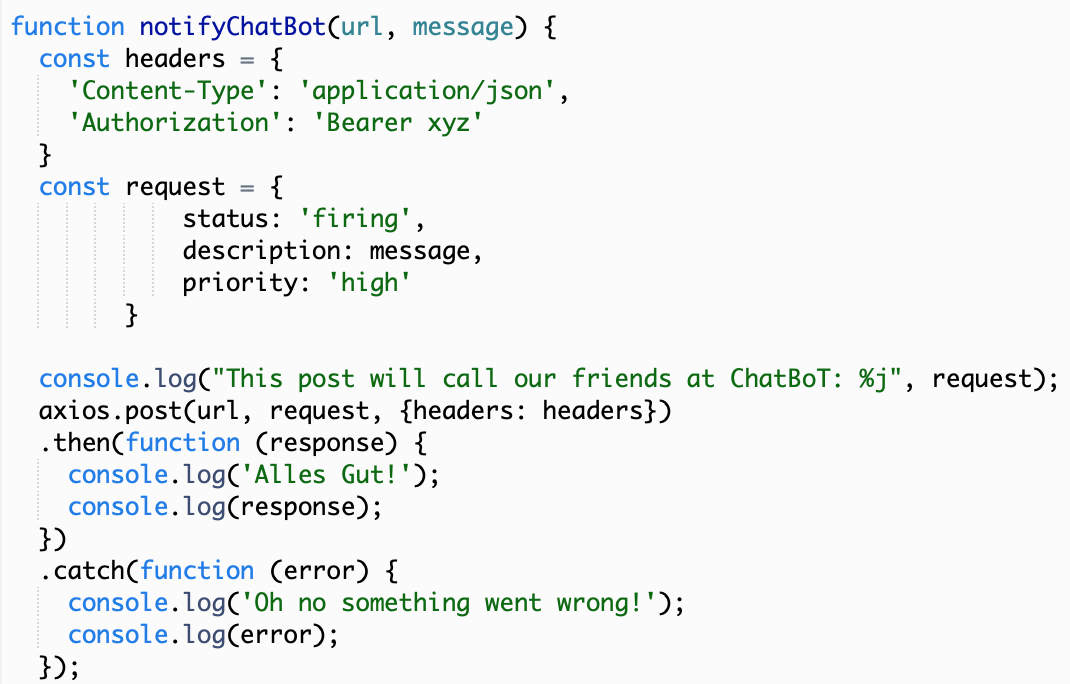
\includegraphics[width=0.85\textwidth]{images/chatbot-api-notif.png}
    \caption{Example of ChatBot API notification}
    \label{fig:chatbot}
\end{figure}


\begin{itemize}
\item \textbf{Slack channel metrics} - To send the message with exact metrics and data we are sending the message to the slack channel using Amazon Simple Notification Service topic.

\begin{lstlisting}[language=Python, caption=Sending message to slack channel using SNS topic]
    #Send Slack MSG
    sns = boto3.resource('sns')
    topic = sns.Topic('arn:aws:sns:us-east-1:746022503515:RCF-SageMaker')
    
    response = topic.publish(
        Message=str("Final Cut-Off Score: {}".format(score_cutoff)),
        Subject='#aws',
        MessageStructure='text/plain',
    )
\end{lstlisting}
\item \textbf{Slack channel graph} - Unfortunately to send the graph to the slack channel method with using SNS topic was not working correctly. For showing the graph using AWS lambda function we needed to do the following steps:

\begin{enumerate}
\item Plot a new graph in memory.
\item Save that graph to a buffer and go to the beginning of a buffer
\begin{lstlisting}[language=Python, numbers=none]
    buf = io.BytesIO()
    plt.savefig(buf, format='png')
    buf.seek(0)
\end{lstlisting}
\item Add a buffer to a structure
\begin{lstlisting}[language=Python, numbers=none]
    my_file = {
    'file' : ('./buf.jpg', buf, 'png')}
\end{lstlisting}

\item Add that structure to the REST POST and post that file to a slack channel.

\begin{lstlisting}[language=Python, numbers=none]
    r = requests.post("https://slack.com/api/files.upload", params=payload, files=my_file)
\end{lstlisting}

\end{enumerate}
\end{itemize}




% Amazon Simple Notification Service - to notify the easiest way.
